\documentclass[aspectratio=169]{beamer}
\usepackage[T1]{fontenc}

%\documentclass[aspectratio=169]{beamer}
%\usetheme{Madrid} % My favorite!
%\usetheme{Boadilla} % Pretty neat, soft color.
%\usetheme{default}
%\usetheme{Warsaw}
%\usetheme{Bergen} % This template has nagivation on the left
%\usetheme{Frankfurt} % Similar to the default 
%\usetheme{Copenhagen}
\usetheme{Goettingen}
%with an extra region at the top.
\usecolortheme{seahorse} % Simple and clean template
%\usetheme{Darmstadt} % not so good
% Uncomment the following line if you want %
% page numbers and using Warsaw theme%
% \setbeamertemplate{footline}[page number]
%\setbeamercovered{transparent}
\setbeamercovered{invisible}
\setbeamersize{text margin right=3.5mm, text margin left=7.5mm}  % text margin
\setbeamertemplate{caption}[numbered]

\setbeamerfont{page number in head/foot}{size=\large}
\setbeamertemplate{footline}[frame number]


% To remove the navigation symbols from 
% the bottom of slides%

\usepackage{graphicx}
\usepackage{epstopdf}
\usepackage{booktabs}
\usepackage{array}
\usepackage{adjustbox}


\renewcommand{\arraystretch}{1.3}
\usepackage{rotating}
\usepackage{pifont}
\usepackage{hyperref}
\usepackage{fontawesome}

\pdfstringdefDisableCommands{
\let\\\space
}



\usepackage{amsmath,amsfonts,amsthm,color,psfrag,epsf, tabularx, multirow, longtable, pdflscape}
\usepackage{pgfplots}
\usepackage{tikz}
\usetikzlibrary{shapes,shapes.misc,arrows,positioning,calc,fit}
\usepackage[
backend=biber,
autocite=superscript,
natbib=true,
style=numeric,
sorting=none]{biblatex}

\addbibresource{Thesis.bib}

\usepackage{pgfplots}
\pgfplotsset{compat=1.13}
\usepackage{tikz}
\usepackage{appendixnumberbeamer}


\usepackage[detect-weight=true, binary-units=true, range-units=single]{siunitx} % Properly Centered numbers in tables

\usetikzlibrary{shapes, graphs, quotes, arrows, backgrounds, positioning, calc}
\usepackage{calc}


\usepackage[caption=false]{subfig}
\usepackage{pifont}
\newcommand*\OK{\ding{51}} % requires pifont


\usepackage{amsmath,amsthm, amssymb, latexsym}
\usepackage{booktabs}
\usepackage{colortbl}
\usepackage{hyperref}
%\usepackage[textsize=tiny]{todonotes}
%\presetkeys{todonotes}{inline}{}

\interdisplaylinepenalty=2500
\hyphenpenalty=10000

\usepackage[english]{babel}
\addto\captionsenglish{\renewcommand{\figurename}{Fig.}}

\def\checkmark{\tikz\fill[scale=0.4](0,.35) -- (.25,0) -- (1,.7) -- (.25,.15) -- cycle;} 
\def\scalecheck{\resizebox{\widthof{\checkmark}*\ratio{\widthof{x}}{\widthof{\normalsize x}}}{!}{\checkmark}}
%that's defined it - now for a test

\makeatletter
\newcommand*{\minuscellcolor}{}
\def\minuscellcolor\ignorespaces{%
% \ignorespaces not really needed, because \@ifnextchar gobbles spaces

\@ifnextchar-{\cellcolor[HTML]{FFAAAA}}{}
}
\newcolumntype{L}{>{\minuscellcolor}l}
\newcolumntype{C}{>{\minuscellcolor}c}
\newcolumntype{R}{>{\minuscellcolor}r}
\makeatother
\newcommand*\rot{\rotatebox{90}}
\tikzset{
block/.style = {draw, fill=white, rectangle, minimum height=3em, minimum width=3em, text width=8em, text centered},
tmp/.style  = {coordinate}, 
sum/.style= {draw, fill=white, circle, node distance=1cm},
input/.style = {coordinate},
output/.style= {coordinate},
pinstyle/.style = {pin edge={to-,thin,black}
},
from/.style args={#1 to #2}{% without transformations
above right={0cm of #1},% needs positioning library
/utils/exec=\pgfpointdiff
{\tikz@scan@one@point\pgfutil@firstofone(#1)\relax}
{\tikz@scan@one@point\pgfutil@firstofone(#2)\relax},
minimum width/.expanded=\the\pgf@x,
minimum height/.expanded=\the\pgf@y},
doc/.style={draw, shape=roundedNode, align=center},
bluefill/.style={fill=blue, opacity=0.5, text opacity=1}
}
\tikzset{
*|/.style={
to path={
(perpendicular cs: horizontal line through={(\tikztostart)},
vertical line through={(\tikztotarget)})
% is the same as (\tikztostart -| \tikztotarget)
% but just to be safe: http://tex.stackexchange.com/a/29781/16595
-- (\tikztotarget) \tikztonodes
}
}
}
\graphicspath{{../Figures/}{../posters/PDW-15/figures/},{./img/}}
\DeclareGraphicsExtensions{.pdf,.png,.jpg}
%\usepackage{bm}         % For typesetting bold math (not \mathbold)
%\logo{\includegraphics[height=0.6cm]{yourlogo.eps}}

\title{Analytical Metric Weight Generation for Multi-Domain Trust in Autonomous Underwater MANETs}

\author[Bolster, A \& Marshall A]{Andrew Bolster and Alan Marshall}
\institute[UoL]
{
University of Liverpool \\
\medskip
{\emph{\{andrew.bolster,alan.marshall\}@liv.ac.uk}}\\
\vspace{0.3in}
\includegraphics[width=0.5\textwidth]{img/livuni}%
}
\date[UComms'16]{UComms 2016, Lerici, Italy}
% \today will show current date. 
% Alternatively, you can specify a date.
%

% If you have a file called "university-logo-filename.xxx", where xxx
% is a graphic format that can be processed by latex or pdflatex,
% resp., then you can add a logo as follows:

% \pgfdeclareimage[height=0.5cm]{university-logo}{university-logo-filename}
% \logo{\pgfuseimage{university-logo}}



% Delete this, if you do not want the table of contents to pop up at
% the beginning of each subsection:
\AtBeginSubsection[]
{
\begin{frame}<beamer>{Outline}
  \tableofcontents[currentsection,currentsubsection]
\end{frame}
}


\begin{document}

\begin{frame}
  \titlepage
\end{frame}

\frame{\tableofcontents}

\section{Background}

\begin{frame}{Ieri, oggi, domani}
  \begin{block}{Ieri}
    Physical Characterisation of Acomms Media, Channel Access Strategies, Centralised Routing Topologies
  \end{block}
  \begin{exampleblock}{Oggi}
    Collaborative access control, Untethered operations, MIMO, (some) Networking Abstractions, Experimental Autonomy, DLL interface standardisation, static-site as a Service (LOON)
  \end{exampleblock}
  \begin{alertblock}{Domani}
    Decentralised local resource coordination, Reactive/Application driven Autonomy, Generalised IP-like abstractions, AUV as a Service?
  \end{alertblock}\pause
  \structure{I hope you guys get this stuff right otherwise I'm stuffed.}
\end{frame}
%

\section{Motivation}

\subsection{Trust}

\begin{frame}{Trust}
  ``the level of confidence one agent has in another to perform a given action on request or in a certain context''\pause
\begin{figure}
	\centering
	  \includegraphics[width=\linewidth]{Trust.jpg}
\end{figure}
\end{frame}

\begin{frame}{Usefulness of Trust in Autonomy}
  \begin{itemize}
    \item Trust vs Security?\pause
    \item Trust vs Autonomy?\pause
    \item Trust vs Formal Verification
  \end{itemize}
\end{frame}

\begin{frame}{Trust Modeling}
	\begin{figure}[h]
		\centering
		\resizebox{\linewidth}{!}{%
		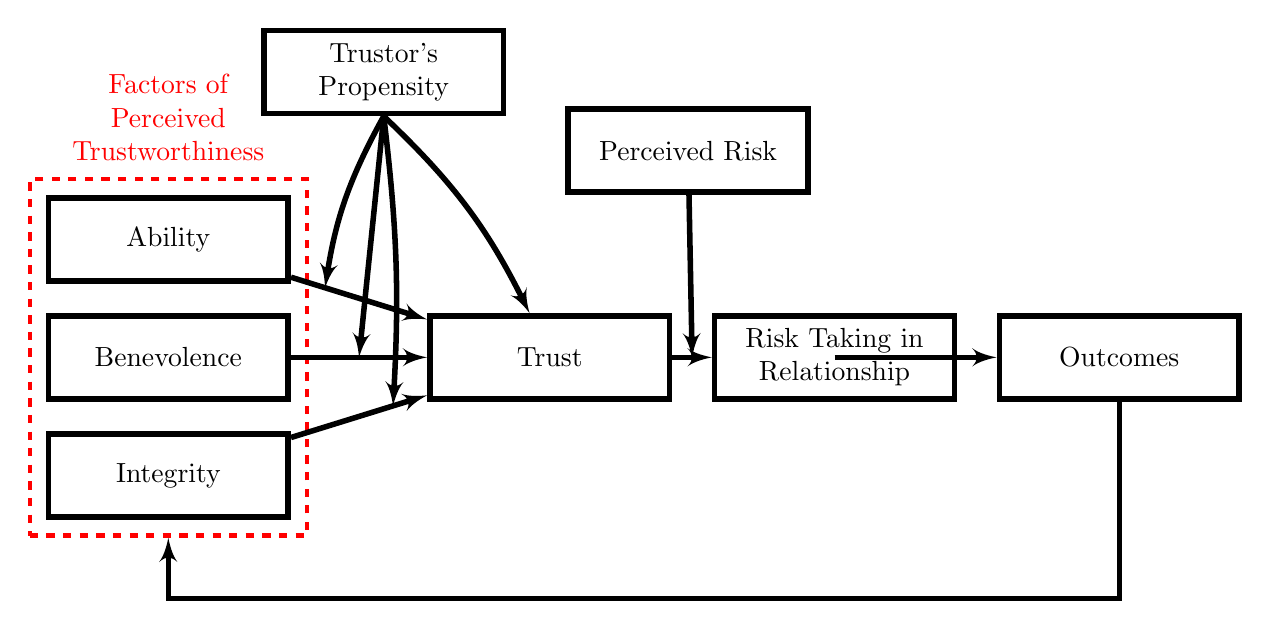
\begin{tikzpicture}[auto, node distance=1.5cm and 0.5cm, line width=2pt, >=latex']
		\node [block] (ability) {Ability};
		\node [block, below of = ability] (benevolence) {Benevolence};
		\node [block, below of = benevolence] (integrity) {Integrity};
		%\draw[red,thick,dotted] ($(ability.north west)+(-0.3,0.6)$)  rectangle ($(integrity.south east)+(0.3,-0.6)$);
		\node (percievedFactors) [draw=red, fit= (ability) (benevolence) (integrity), inner sep=0.2cm, dashed, ultra thick, fill opacity=0.2] {};
		\node [yshift=5ex, red, text width=8em, text centered] at (percievedFactors.north) {Factors of Perceived Trustworthiness};
		
		\node [block, right=1.5cm and 1.5cm of percievedFactors] (trust) {Trust};
		
		\node [block, above=2.5cm of trust, xshift=-6em] (trustorsPropensity) {Trustor's Propensity};
		\node [block, right=of trust] (riskTaking) {Risk Taking in Relationship};
		\node [block, above=of trust, xshift=5em] (percievedRisk) {Perceived Risk};
		\node [block, right=of riskTaking] (outcomes) {Outcomes};
		
		\draw [->] (ability) --coordinate[near start](mAb)  (trust);
		\draw [->] (benevolence) -- coordinate[midway](mBe) (trust);
		\draw [->] (integrity) -- coordinate[near end](mIn) (trust);
		\draw [->] (trustorsPropensity.south) to[bend right=10] (mAb);
		\draw [->] (trustorsPropensity.south) to (mBe);
		\draw [->] (trustorsPropensity.south) to[bend left=5] (mIn);
		\draw [->] (trustorsPropensity.south) to[bend left=10] (trust);
		\draw [->] (trust) -- coordinate[midway](mT) (riskTaking);
		\draw [->] (percievedRisk) -- (mT);
		\draw [->] (riskTaking) |- (outcomes);
		\draw [->] (outcomes.south) --++ (0cm,-2.5cm) -| (percievedFactors.south);
		
		\end{tikzpicture}
		}
		\caption[Model of Trust]{Model of Trust (from~\citet{Mayer1995})}
		\label{fig:mayer_trust_model}
	\end{figure}
\end{frame}

\begin{frame}{Context}
	\begin{figure}
		\includegraphics[width=\linewidth]{auto_nets.jpg}
	\end{figure}
\end{frame}

\begin{frame}{Context}
  % - A title should summarize the slide in an understandable fashion
  %   for anyone how does not follow everything on the slide itself.

  \begin{itemize}
    \item
	  Trust is useful in Ad-hoc/distributed/decentralised nets
    \item
      Trust Management Frameworks (TMFs) require reassessment in UWA
    \item 
      Most rely on one type of observation (metric) (PLR)
    \item 
      Recent work\autocite{Guo11} fuses multiple metrics for assessment.
      \pause
    \item
      What metrics are suitable for use underwater?
    \item 
      How do MANET Single and Multi-Metric Frameworks perform in UWA? \autocite{Bolster2015}\pause \alert{ badly}\pause \alert{, but multi can just about survive}\pause
    \item
      \structure{How to robustly optimise multi-metric/domain abstraction?}\pause \alert{ and is it worthwhile?}
  \end{itemize}
\end{frame}



\subsection{Related Work}

\begin{frame}{Trust in Conventional RF MANETS}
  \begin{itemize}
    \item 
      TMFs provide information to assist the estimation of future states and actions of nodes within networks.
    \item
      Centralised methods unsuitable for dynamic networks in terms of efficiency and robustness\autocite{Caiti2011}.
    \item 
      Need to detect, identify, \& mitigate threats in a distributed fashion.
  \end{itemize}
\end{frame}

\begin{frame}{Single-Metric TMFs}
  Most can be generalised as single-value estimations of PLR/Successful Routes, with the incorporation of some \emph{meta}-observations e.g. Topology
  \begin{itemize}
    \item \emph{Hermes} \autocite{Zouridaki2005} - Bayesian estimation based on PLR
    \item \emph{OTMF} \autocite{Li2008} - Collaborative Bayesian Trust
    \item \emph{TSR} \autocite{Moe2008a} - HMM route assessment, Session Loss Rate.
    \item \emph{CONFIDANT} \autocite{Buchegger2002} - Probabilistic PLR assessment, inc. topology \& reputation weighting.
    \item \emph{Fuzzy Trust-Based Filtering} \autocite{Luo2008} - Fuzzy classification of packet delivery
  \end{itemize}
\end{frame}
\begin{frame}{Single-Metric TMFs}
  \begin{itemize}
    \item
      Opportunities for malicious actors to undermine the operation of a network. 
    \item 
      Not an issue in networks where Comms.\ is the primary operating concern, but is significant in resource constrained environments \pause \alert{like UWA}
  \end{itemize}
\end{frame}

\begin{frame}{Multi-Metric TMF} 
  \emph{Multi-metric Trust For MANETS (MTFM)} \autocite{Guo11} 
  \begin{itemize}
    \item Additional metrics as well as PLR, 
    \item Topological relationship,
    \item Metric weighting enables behaviour classification
    \item Grey Relational Grading 
      \begin{itemize}
        \item dynamic runtime normalisation, assessing \structure{comparative} trust within a cohort of actors.
      \end{itemize}
  \end{itemize}
  \pause
  \centering
  Operates favourably in RF against OTMF and Hermes, accurately detecting, identifying, \& characterising misbehaviours.\autocite{Guo11}
  \pause
  \centering
  Turns out it is ``not as bad as the rest'' in UWAN.\autocite{Bolster2015}  
\end{frame}

\begin{frame}{Multi-Metrics Comms TMF performance}
	\begin{figure}
		\centering
		\includegraphics[width=\textwidth]{trust_beta_otmf_mtfm_boxes}
		\label{fig:otmf_beta_comparison_boxes}
	\end{figure}
	\structure{MTFM 0.5 baseline bias vs OTMF/Hermes optimism}
\end{frame}

\subsection{Challenges to Trust in Underwater Networks}

\begin{frame}{Operational Considerations: Collaborative AUV Survey}
  \begin{columns}
    \begin{column}{0.5\textwidth}
      Context:
      \begin{itemize}
        \item Fleets of up to 16 collaborating Autonomous Underwater Vehicles(AUVs) (not ``Swarms'')
        \item Constrained in Power, Mobility, Processing, Storage Capacity
        \item Tasked to perform ongoing survey of an area
      \end{itemize}

      \uncover<2->{\centering
      Communications Efficiency is not the only factor at risk from malicious exploitation}
    \end{column}
    \begin{column}{0.5\textwidth}
      \begin{figure}[h]
        \begin{center}
          \includegraphics[width=\linewidth]{remus100cmre}
        \end{center}
        \caption{REMUS 100 AUV as deployed at NATO CMRE La Spezia}
        \label{fig:remus100cmre}
      \end{figure}

    \end{column}
  \end{columns}
\end{frame}

\begin{frame}{Threat Surface}
  \begin{figure}[h!]
    \centering
    \includegraphics[width=\linewidth]{threat_surface_sum}
    \caption[Multi-Domain Threat Surface]{Multi-Domain Threat Surface}
    \label{fig:threat_surface}
  \end{figure}

  \pause
  Current trust methods monitor a \alert{tiny} area of the potential threat surface
\end{frame}



\section{Our Contribution}

\subsection{Multi-Metric Trust Assessment}


\begin{frame}{Multi-Metric Weighted Trust with Grey relations}

  \begin{align}
    \theta_{k,j}^t &= \frac{\min_k|a_{k,j}^t - g_j^t| + \rho \max_k|a_{k,j}^t-g_j^t|}{|a_{k,j}^t-g_j^t| + \rho \max_k|a_{k,j}^t-g_j^t|} \\
    \phi_{k,j}^t &= \frac{\min_k|a_{k,j}^t - b_j^t| + \rho \max_k|a_{k,j}^t-b_j^t|}{|a_{k,j}^t-b_j^t| + \rho \max_k|a_{k,j}^t-b_j^t|} \\
    [\theta_k^t, \phi_k^t] &= \left[\sum_{j=0}^M h_j \theta_{k,j}^t,\sum_{j=0}^M h_j \phi_{k,j}^t \right] \\
    T_k^t &= ({1+{(\phi_k^t)^2}/{(\theta_k^t)^2}})^{-1} 
  \end{align}

  Where  $a_{k,j}^t$ is the value of an observed metric $x_j$ for a given node $k$ at time $t$,  $g$ and $b$ are respectively the ``good'' and ``bad'' reference metric sequences from $\{a_{k,j}^t k=1,2\dots K\}$, $H=[h_0\dots h_M]$ is a metric weighting vector such that $\sum h_j = 1$
\end{frame}

\begin{frame}{Factor of Opportunity in Trust Assessment}
  \begin{block}{Weight}
    $H = [h_j \forall j in [0\cdots M]]$

    Relative importance of a given metric $j$
  \end{block}

  \begin{block}{Valence}
    $g_j \mapsto max , b_j \mapsto min $ VS
    $g_j \mapsto min , b_j \mapsto max $

    Is this metric $j$ positively or negatively related to Trust? 
  \end{block}


\end{frame}

\begin{frame}{Optimisation vector of Trust assessment}
  \begin{block}{Trust assessment of misbehaving node should be:}
    \begin{enumerate}
      \item maximally deviant wrt. ``fair'' nodes
      \item identified as ``low''
    \end{enumerate}
  \end{block}
  \pause
  \begin{block}{Objective Functions}
    \begin{align}
      \Delta T_{ix} &= \frac{\sum_{j\neq x}\left( \overline{T_{i,j}}^{\forall t}\right)}{N-1} - \overline{T_{i,x}}^{\forall t} \label{eq:delta_t}\\
      \Delta T_{ix}^- &= \frac{\sum_{j\neq x} \Delta T_{ij}}{N-1} - \overline{\Delta T_{i,x}}^{\forall t} \label{eq:delta_t_minus} 
    \end{align}

  \end{block}
\end{frame}

\begin{frame}{Parameter Regression and Optimisation}
  \begin{block}{Proposed General Methodology}
    Assess the relative importance of metrics in differentiating between behaviours using Random Forest Ensemble regression.

    Constrained iterative solution space for valence enumeration.
  \end{block}
\end{frame}


\begin{frame}{Metric Domains}
  \begin{block}{Communications}
    \begin{equation}
      X_{comms}=\{D, P_{RX}, P_{TX}, S, G, PLR\}
    \end{equation}
  \end{block}

  \pause
  \begin{block}{Physical}
    \begin{align}
      \centering
      INDD_{i,j} &= \frac{|P_j - \sum_x \frac{P_x}{N}|}{\frac{1}{N}\sum_x \sum_y{|P_x - P_y| (\forall x \neq y)}}\\
      INHD_{i,j} &= \hat{v} \vert v= V_j - \sum_x{\frac{V_x}{N}}\\
      V_{i,j} &= |V_j|\\
      X_{phy}&=\{\text{INDD}, \text{INHD}, V\}
    \end{align}
  \end{block}

\end{frame}

\begin{frame}{Multi-domain Metric Vector}
  Simplest possible combination; vector concatenation across domains 

  \begin{align}
    \centering
    X_{merge} &=  (X_{comms}|X_{phy}) \nonumber\\
    &= \{D, P_{RX}, P_{TX}, S, G, PLR, \text{INDD}, \text{INHD}, V\}
    \label{eq:merge:vector}
  \end{align}

  \pause 

  \alert{Not all metrics created equally}

  (or equally relevant to specific behaviours)
\end{frame}



\subsection{Experimental Context}

\begin{frame}{Scaling Considerations}
  \begin{figure}[h]
    \centering
    \subfloat[][All Nodes Static]{\includegraphics[width=0.35\linewidth]{2d_ratio_static.pdf}}
    \subfloat[][$n_1$ Random Walk]{\includegraphics[width=0.35\linewidth]{2d_ratio_single_mobile.pdf}}\\
    \subfloat[][All nodes but $n_1$ Random Walk]{\includegraphics[width=0.35\linewidth]{2d_ratio_allbut1.pdf}}
    \subfloat[][All nodes Random Walk]{\includegraphics[width=0.35\linewidth]{2d_ratio_all_mobile.pdf}}
    \label{fig:CommsThroughputRatios}
  \end{figure}


\end{frame}

\begin{frame}{Misbehaviour Specification}
  \begin{alertblock}{Assumptions}
    \begin{itemize}
      \item Consistent misbehaviour
      \item Single misbehaver
      \item Honest position reporting \structure{(/Collaborative Localisation?)}
    \end{itemize}
  \end{alertblock}
  %
  \begin{block}{Misbehaviours of $n_a$}
    \begin{itemize}
      \item \emph{Malicious Power Control}(MPC) - attacker makes $n_t$ appear selfish by ++ power $n_i \forall i\neq t$
      \item \emph{Selfish Target Selection}(STS) - node preferentially communicates with nodes close to it.
      \item \emph{Shadowing} - follows with no mission knowledge.
      \item \emph{SlowCoach} - `misbehaver` with simulated prop. fouling 
    \end{itemize}
    Base Behaviour: Port protection pattern with dynamic Boidean collision avoidance / flocking.

  \end{block}

\end{frame}



\begin{frame}[label=scaling]{Scaling Considerations}
  \begin{itemize}
    \item Simulations based on SimPy \autocite{Mueller2003SimPy}, Network stack using AUVNetSim \autocite{Miquel2008} and channel constraints based on Stojaovic and Stefanov \autocite{Stojanovic2007,Stefanov2011}\hyperlink{tab:sysconstraints}{\beamergotobutton{Details}}
      \pause
    \item Established a safe operating zone optimising for delay/throughput  \hyperlink{eq:networkeffects}{\beamergotobutton{Details}}
    \item Six per-link communications metrics
      \pause
      \begin{columns}
        \begin{column}{0.5\textwidth}
          \begin{itemize}
            \item Received Power
            \item Received Throughput
            \item E2E Delay
          \end{itemize}
        \end{column}
        \begin{column}{0.5\textwidth}
          \begin{itemize}
            \item Transmitted Power
            \item Transmitted Throughput
            \item Packet Loss Rate
          \end{itemize}
        \end{column}
      \end{columns}
  \end{itemize}

\end{frame}


\subsection{Metric Significance}
\begin{frame}{Regression of Metric Significance}
  Aim: Establish which metrics are important in discriminating behaviours
  \pause
  \begin{itemize}
    \item Distributed Random Forest Regression \autocite{Breiman2001} 
    \item 18661 Metric Weight Vectors ($H(X_{\text{merge}})$), 512 random trees
    \item 16 Random starts of each of the 4 misbehaving scenarios for 6 nodes for 6 hour ``missions''
    \item 32 Random starts of each of the ``fair'' mission
    \item Regression identifies the significance of metrics in classifying between the possible behaviours + ``fair''
  \end{itemize}

\end{frame}
\begin{frame}{Metric Significance}

  \begin{figure}[h!]
    \centering

    \includegraphics[width=0.6\linewidth]{full_metric_trust_relevance}
    \caption{Multi Domain  Metric Features ($X_{merge}$)}
    \label{fig:multi_feature_extraction}
  \end{figure}
  \pause
  Brute force valence search with $R>0.1 \mapsto $ massive reduction in complexity space
\end{frame}

\begin{frame}{Also apply to specific domains for comparison}
  i.e. $X_{\text{comms}},X_{\text{phys}}$
  \pause
  \begin{table}
    \centering
    \caption{$\Delta T$ across domains and detected behaviours}
    \begin{tabular}{l*{4}{c}r}
      \toprule
      \multirow{2}{*}[-2pt]{Domain} & \multicolumn{4}{c}{Behaviour}&\multirow{2}{*}[-2pt]{Avg.}\\ \cmidrule(r){2-5}
      &  MPC &  STS &  Shadow &  SlowCoach & \\
      \midrule
      $X_{merge}$& 0.90 & 0.10 &    0.50 &       0.63 &  0.53 \\
      $X_{comms}$& 0.95 & 0.17 &    0.28 &       0.27 &  0.42 \\
      $X_{phys}$ & 0.02 & 0.02 &    0.43 &       0.76 &  0.31 \\
      \hline
      Avg.       & 0.67 & 0.10 &    0.41 &       0.56 &  0.44 \\
      \bottomrule
    \end{tabular}
    \label{tab:domain_deltas}
  \end{table}
\end{frame}

\begin{frame}{That's nice but what does it mean?}
	
	
	\begin{figure}[h]
		\centering
		\subfloat[Comms. Metric Trust Response\label{fig:comms_slowcoach}]{%
			\includegraphics[width=0.5\linewidth]{best_comms_run_SlowCoach}
		}
		\subfloat[Full Metric Trust Response\label{fig:full_slowcoach}]{%
			\includegraphics[width=0.5\linewidth]{best_full_run_SlowCoach}
		}
		\caption{Trust Responses for SlowCoach using domain-optimised weights}
	\end{figure}\pause
	\alert{Misbehaviours are more eaily descernible when weighted}
\end{frame}

\begin{frame}{\alert{FYI} Detection Characteristics}
  \begin{table}
    \centering
    \resizebox{\linewidth}{!}{%

    \begin{tabular}{|l||r|r|r|r|r|r|r|r|}
      \toprule
      \multirow{3}{*}{Domain} &    \multicolumn{4}{c|}{\parbox{4cm}{\centering True Positive Identification of Misbehaver\vspace{.5\baselineskip}}} &    \multicolumn{4}{c|}{\parbox{4cm}{\centering False Positive Identification of Misbehaver\vspace{.5\baselineskip}}}    \\[0.3em]
      &   \rot{MPC} &  \rot{STS} & \rot{Shadow} & \rot{SlowCoach} &   \rot{MPC} &  \rot{STS} & \rot{Shadow} & \rot{SlowCoach} \\
      \midrule
      Full          &  1.00 &  0.03 &   0.63 &      0.98 &  0.00 &  0.07 &   0.00 &       0.0 \\
      Comms         &  1.00 &  0.05 &   0.18 &      0.39 &  0.00 &  0.03 &   0.04 &       0.0 \\
      Phys          &  0.03 &  0.02 &   0.40 &      0.85 &  0.12 &  0.09 &   0.00 &       0.0 \\
      \bottomrule
    \end{tabular}
    }
    \caption{Accuracy of Correct identification of misbehaver using Domain-Trained weight vectors with a Dixons Q based limit-classifier}
    \label{tab:synth_detect}
  \end{table}
\end{frame}

\begin{frame}{More stuff not in the paper but FYI}
  \structure{Are our domain assumptions useful? Are there better ways to group metrics/behaviours?}

  \begin{figure}[h]
    \centering
	\begin{adjustbox}{max totalsize={.9\textwidth}{.7\textheight},center}
	
    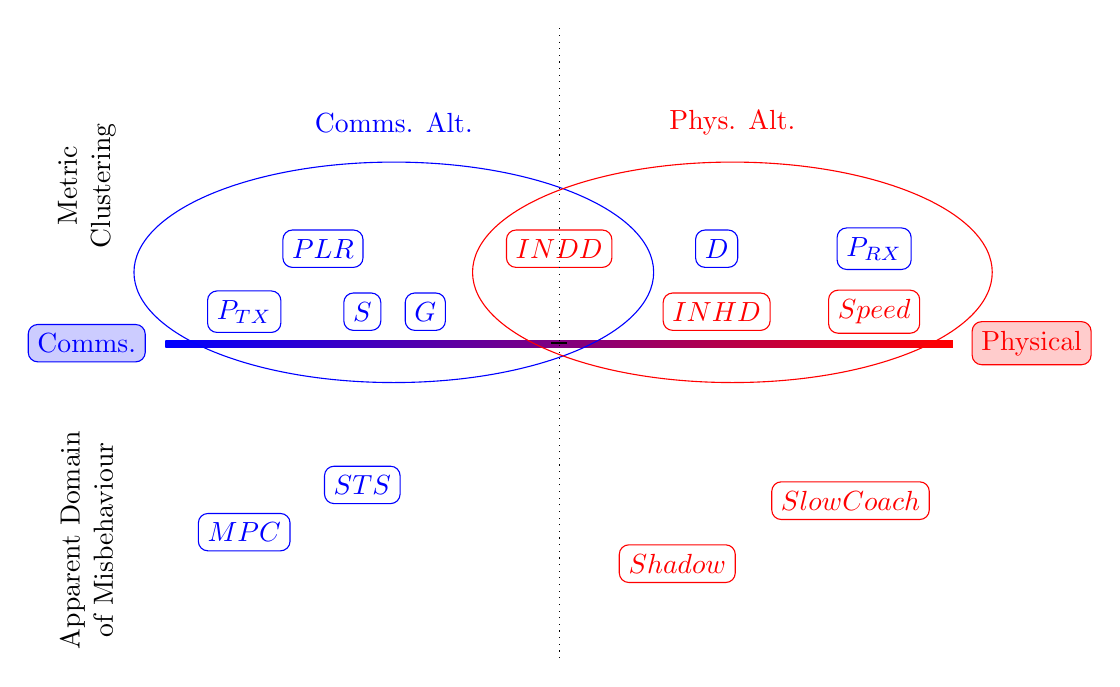
\begin{tikzpicture}[-latex,
      comms/.style={text=blue, draw=blue, rounded corners=.8ex},
      phys/.style={text=red, draw=red, rounded corners=.8ex}]
      % Start off with the line
      %\draw [<-|][comms, draw=blue, very thick] (0,1) -- (5,1); 
      %\draw [|->][phys, draw=red, very thick] (5,1) -- (10,1); 
      \path[left color=blue,right color=red]
      (0,0.95) rectangle +(10,2.5pt);

      % Baseline labels
      \node[comms, fill=blue, fill opacity=0.2, text opacity=1] at (-1,1) {Comms.};
      \node[phys, fill=red, fill opacity=0.2, text opacity=1] at (11,1) {Physical};

      % Metric Labels
      \node[comms] at (7,2.2) {$D$};
      \node[comms] at (9,2.2) {$P_{RX}$};
      \node[comms] at (1,1.4) {$P_{TX}$};
      \node[comms] at (2.5,1.4) {$S$};
      \node[comms] at (3.3,1.4) {$G$};
      \node[comms] at (2,2.2) {$PLR$};
      \node[phys] at (5,2.2) {$INDD$};
      \node[phys] at (7,1.4) {$INHD$};
      \node[phys] at (9,1.4) {$Speed$};

      \node[rotate=90, align=center] at (-1, 3) {Metric\\Clustering};
      \node[rotate=90, align=center] at (-1, -1.5) {Apparent Domain\\of Misbehaviour};
      \node[comms] at (1,-1.4) {$MPC$};
      \node[comms] at (2.5,-0.8) {$STS$};
      \node[phys] at (6.5,-1.8) {$Shadow$};
      \node[phys] at (8.7,-1) {$SlowCoach$};

      % Draw approx subsets
      \draw[comms] (2.9,1.9) ellipse (3.3 and 1.4);
      \draw[phys] (7.2,1.9) ellipse (3.3 and 1.4);

      \node[text=red] at (7.2,3.8) {Phys. Alt.};
      \node[text=blue] at (2.9,3.8) {Comms. Alt.};

      % Misc
      \draw[-|][dotted] (5,5) -- (5,1);
      \draw[-|][dotted] (5,-3) -- (5,1);


    \end{tikzpicture}
    \end{adjustbox}
    \caption{Possible Alternate Metric Domain Groupings?}
    \label{fig:alternate_domain_diag}
  \end{figure}
\end{frame}



\begin{frame}{What about going to extremes?}

  \begin{figure}
    \centering
    \includegraphics[width=\linewidth]{positive_heat}
    \caption{Accuracy of Correct identification of misbehaver using Domain-Trained weight vectors with a Dixons Q based limit-classifier}
    \label{fig:positive_heat}
  \end{figure}

\end{frame}
\begin{frame}{Key Observations}
  \begin{itemize}
    \item PLR not the most useful metric in \alert{discriminating} behaviours
      \pause\item Combination of Significance and Correlations provide selectivity
      \pause\item MTFM has capability to finely discriminate between similar misbehaviours
      \pause\item Identifying this classification ``comb'' is computationally intensive and grows exponentially with number of metrics involved for brute force regression
      \pause\item Use of Ensemble ML method and relevance filtering $=$ Practical Real-time training
      \pause\item High \structure{simulated} selectivity depending on behaviour class
  \end{itemize}
\end{frame}


\section*{Summary}

\begin{frame}{Done}
  % Keep the summary *very short*.
  
\begin{block}{$\Delta$}
   	\begin{itemize}
   		\item UWA Multi Metric Comms Trust
   		\item Detection of non-comms misbehaviours/fouling \structure{even just using comms metrics}
   		\item Methodology for exploring / training / metric relevance
   		\item Minimal performance specification
   	\end{itemize}
\end{block}

  \begin{block}{$\Sigma$}
    \begin{itemize}
      \item UWA Trust is \alert{Hard} \& it's mostly the channels' fault
      \item Single-Metric Trust is \alert{unstable} in such an environments
      \item Multi-Metric Trust works \& can \alert{discriminate behaviours}
      \item \alert{Not all metrics} are equally useful
      \item Simple classifiers \alert{can} be V good in \alert{some} behaviours
    \end{itemize}
  \end{block}
\end{frame}

\begin{frame}{Left/Next}
  \begin{alertblock}{$\notin$}
    \begin{itemize}
      \item Smarter Detection Classifier
      \item Cooperative / Periodic / Variable attack profiles
      \item Commonality of detection filters across Multiple-base scenarios
      \item Heterogenous Node capabilities\pause
      \item \alert{Real} experiments and Cross sim-implementations
    \end{itemize}
  \end{alertblock}


  \pause
    \begin{exampleblock}{$\mathop{\mathbb{E}}$}
    	\begin{itemize}
    		\item Network that works
    		\item Stable Abstractions / Interoperability
    		\item \alert{reflective autonomy}
    	\end{itemize}
    \end{exampleblock}

\end{frame}

\begin{frame}[t,allowframebreaks]
  \frametitle{References}
  \printbibliography[title=References]% [nottype=video]}
\end{frame}

\begin{frame}{\alert{Thank You / QnA?}}
          \begin{center}
          	\begin{minipage}{4cm}
\begin{exampleblock}{Say Hello!}
	\begin{itemize}
		\item[\faEnvelope] \href{mailto:bolster@liv.ac.uk}{bolster@liv.ac.uk}
		\item[\faEnvelope] \href{mailto:me@bolster.online}{me@bolster.online}
		\item[\faTwitter] \href{https://twitter.com/bolster}{@bolster}
		\item[\faSitemap] \href{http://bolster.online}{bolster.online}
		\item[\faGithub] \href{https://github.com/andrewbolster}{andrewbolster}
		\item[\faLinkedin] \href{http://www.linkedin.com/in/andrewbolster}{''Andrew Bolster''}
		\item[\faStackOverflow] \href{http://www.stackoverflow.com/users/252556/bolster}{bolster}
	\end{itemize}
\end{exampleblock}
\end{minipage}
\end{center}
\end{frame}

\appendix

\begin{frame}{Communications Channel Considerations}
  Key Characteristics of the Marine Acoustic Channel \autocite{Urick1983a,Partan2006,Stojanovic2007,Stefanov2011}:
  \begin{itemize}
    \item Slow propagation ($~1400ms^{-1}$) incurring long delays
    \item Inter-symbol interference
    \item Doppler Spreading
    \item Non-Linear propagation due to refraction
    \item Fast \& Slow fades from environmental factors (flora/fauna/surface and seabed conditions)
    \item Freq. dependant attenuation
    \item Significant destructive multipath effects
  \end{itemize}

\end{frame}

\begin{frame}{Attenuation in the Marine Acoustic Channel}

  The attenuation that occurs in an underwater acoustic channel over distance $d$ about frequency $f$ is given as $A_{\text{aco}}(d,f) = A_0d^ka(f)^d$ or
  %
  \begin{equation}
    \label{eq:acoattenuationdb}
    10 \log A_{\text{aco}}(d,f)/A_0 = k \cdot 10 \log d + d \cdot 10 \log a(f)
  \end{equation}
  %
  where $A_0$ is a normalising constant, $k$ is a spreading factor, and $a(f)$ is the absorption coefficient\autocite{Stefanov2011};
  %
  \begin{equation}
    \label{eq:thorp}
    10 \log a(f) = \frac{0.11 \cdot f^2}{1+f^2} + \frac{44\cdot f^2}{4100+f^2}+ 2.75\times10^{-4} f^2 + 0.003
  \end{equation}

  \pause

  Compared to RF Free space PL: $(A_{\text{RF}}(d,f) \approx \left( \frac{4\pi d f}{c} \right)^2)$
  \begin{itemize}
    \item \alert{Exponential} in $d$: $A_{\text{aco}} \propto f^{d}$ vs $A_{\text{RF}} \propto (df)^2$
    \item $f$ factor \alert{four orders higher} in $f\propto A_{\text{aco}}$ vs $f\propto A_{\text{RF}}$

  \end{itemize}

\end{frame}

\begin{frame}{Multi-Metric TMF - Grey Grading} 
  \begin{equation}
    \label{eq:grcg}
    \theta_{k,j}^t = \frac{\min_k|a_{k,j}^t - g_j^t| + \rho \max_k|a_{k,j}^t-g_j^t|}{|a_{k,j}^t-g_j^t| + \rho \max_k|a_{k,j}^t-g_j^t|} 
  \end{equation}
  \begin{equation}
    \label{eq:grcb}
    \phi_{k,j}^t = \frac{\min_k|a_{k,j}^t - b_j^t| + \rho \max_k|a_{k,j}^t-b_j^t|}{|a_{k,j}^t-b_j^t| + \rho \max_k|a_{k,j}^t-b_j^t|} 
  \end{equation}
  \begin{equation}
    \label{eq:grc}
    [\theta_k^t, \phi_k^t] = \left[\sum_{j=0}^M h_j \theta_{k,j}^t,\sum_{j=0}^M h_j \phi_{k,j}^t \right]
  \end{equation}
  \begin{equation}
    \label{eq:grcT}
    T_k^t = ({1+{(\phi_k^t)^2}/{(\theta_k^t)^2}})^{-1}
  \end{equation}

  Where  $a_{k,j}^t$ is the value of an observed metric $x_j$ for a given node $k$ at time $t$,  $g$ and $b$ are respectively the ``good'' and ``bad'' reference metric sequences from $\{a_{k,j}^t k=1,2\dots K\}$, $H=[h_0\dots h_M]$ is a metric weighting vector such that $\sum h_j = 1$

\end{frame}
\begin{frame}{Multi-Metric TMF - Topological Relationships} 
  \centering
  Includes shared assessments from other nodes weighted based on their relative topology to provide a final value\footnotemark  

  \vspace{9pt}

  $T_{i,j}^{MTFM}$
  \begin{figure}[h]
    \centering
    \includegraphics[width=.9\textwidth]{node_relationships}
    \label{fig:node_relationships}
  \end{figure}
  \footnotetext{\hyperlink{eq:networkeffects}{\beamergotobutton{Details}}}

\end{frame}


\begin{frame}[allowframebreaks]{Grey Trust Equs}
  \begin{align}
    \label{eq:networkeffects}
    T_{i,j}^{MTFM}=&\frac{1}{2} \cdot \max_s\{f_s(T_{i,j})\} T_{i,j}\\ \notag
    +&\frac{1}{2} \frac{2|N_R| }{2|N_R| + |N_I|}\sum_{n \in N_R} \max_s\{f_s(T_{i,n})\} T_{i,n}\\ \notag
    +&\frac{1}{2} \frac{|N_I| }{2|N_R| + |N_I|}\sum_{n \in N_I} \max_s\{f_s(T_{i,n})\} T_{i,n} 
  \end{align}

  Where $T_{i,n}$ is the subjective trust assessment of $n_i$ by $n_n$, and $f_s = [ f_1,f_2, f_3]$ given as...

  \framebreak

  \begin{align}
    \label{eq:whitenization}
    f_1(x)&= -x+1\notag\\
    f_2(x)&= 
    \begin{cases}
      2x & \text{if }x\leq 0.5\\
      -2x+2 & \text{if }x>0.5
    \end{cases}\\
    f_3(x)&= x\notag
  \end{align}
  \hyperlink{fig:node_relationships}{\beamergotobutton{Back}}
\end{frame}

\begin{frame}[allowframebreaks]{Comms Scaling Graphs}

  \setcounter{subfigure}{0}% Reset subfigure counter
  \begin{figure}[bp!]\centering
    \subfloat[][Packet Delivery]{\includegraphics[width=0.5\linewidth]{emission_throughput_performance_bella_all_mobile}}
    %
    \subfloat[][Probability of arrival]{\includegraphics[width=0.5\linewidth]{emission_prod_breakdown_bella_all_mobile}}\\
    \subfloat[][End to End Delay]{\includegraphics[width=0.5\linewidth]{emission_delay_variation_bella_all_mobile}}
    \subfloat[][RTS Ratios]{\includegraphics[width=0.5\linewidth]{emission_rts_ratio_bella_all_mobile}}
  \end{figure}

  \hyperlink{scaling}{\beamergotobutton{Back}}

\end{frame}

\begin{frame}[shrink]{System Model Constraints}
  \centering
  \begin{table}[h]
    \caption{Comparison of system model constraints as applied between Terrestrial and Marine communications
    \hyperlink{scaling}{\beamergotobutton{Back}}
    } \label{tab:sysconstraints}
    \begin{center}
      \setlength{\tabcolsep}{8pt}
      \begin{tabular}{lccc}
        \toprule
        Parameter & Unit & Terrestrial & Marine \\
        \midrule
        Simulated Duration & $s$ & 300 & 18000\\
        Trust Sampling Period & $s$ & 1 & 600 \\
        Simulated Area & $km^2$ & 0.7 & 0.7-4 \\
        Transmission Range & $km$ & 0.25 & 1.5 \\
        Physical Layer & & RF(802.11) & Acoustic\\
        Propagation Speed& $m/s$ & $3\times10^8$ & 1490\\
        Center Frequency& $Hz$ & $2.6\times10^9$ & $2 \times 10^4$ \\
        Bandwidth& $Hz$ & $22\times10^6$ & $1\times10^4$\\
        MAC Type & & CSMA/DCF & CSMA/CA\\
        Routing Protocol & & DSDV & FBR \\
        Max Speed & $ms^{-1}$ & 5 & 1.5 \\
        Max Data Rate & $bps$ & $5\times10^6$ & $\approx 240$ \\
        Packet Size & bits & 4096 &  9600 \\
        Single Transmission Duration & $s$ & 10 & 32 \\
        Single Transmission Size & bits & $10^7$ & $9600$ \\
        \bottomrule
      \end{tabular}
      \setlength{\tabcolsep}{6pt}
    \end{center}
  \end{table}

\end{frame}

\begin{frame}{Metric Selection/Weighting}
  \begin{table}
    \centering

    \caption{$\Delta T_{ix}$ behaviour detection performance across meta-domains, including selected metrics}
    \resizebox{\linewidth}{!}{%
    \begin{tabular}{c p{2cm}||*{5}{c|}|*{9}{c|}}
	  \toprule
      \multicolumn{2}{|c||}{\multirow{3}{*}{\parbox{2cm}{Domain}}}&\multicolumn{5}{c||}{Behaviour $\Delta T_{ix}$} & \multicolumn{9}{c|}{Metrics in Domain}\\
      &&                \rot{MPC} &  \rot{STS} & \rot{Shadow} & \rot{SlowCoach} & \rot{Mean} &                     \rot{$Delay$} & \rot{$P_{RX}$} & \rot{$P_{TX}$} &  \rot{$S$} &  \rot{$G$} & \rot{$PLR$} & \rot{$INDD$} & \rot{$INHD$} & \rot{$Speed$} \\
      \midrule
      \multirow{3}{*}{\rot{Basic}} & Full       & 0.81 & -0.03 &    0.42 &       0.60 &  0.45 &\OK&\OK&\OK&\OK&\OK&\OK&\OK&\OK&\OK\\
      & Comms      & 0.85 &  0.04 &    0.19 &       0.26 &  0.34 &\OK&\OK&\OK&\OK&\OK&\OK&&&\\
      & Phys       & 0.04 &  0.00 &    0.39 &       0.69 &  0.28 &&&&&&&\OK&\OK&\OK\\\hline
      \multirow{4}{*}{\rot{Alternate}}&&&&&&&&&&&&&&&\\[-0.8em]
      & Comms alt. & 0.85 &  0.03 &    0.38 &       0.45 &  0.43 &&&&\OK&\OK&\OK&\OK&&\\[0.2em]
      & Phys alt.  & 0.48 &  0.03 &    0.42 &       0.63 &  0.39 &\OK&\OK&&&&&\OK&\OK&\OK\\
      &&&&&&&&&&&&&&&\\[-0.5em]\hline
      \multirow{5}{*}{\rot{Synthetic}}&&&&&&&&&&&&&&&\\[-1em]
      & MPC        & 0.89 &  0.01 &   0.35 &      0.54 & 0.45 &                         \OK &      \OK &      \OK &      &      &       &        &    \OK &         \\
      & STS        & 0.86 & 0.06 &   0.37 &      0.49 & 0.45 &                         \OK &          &      \OK &  \OK &      &   \OK &    \OK &        &         \\
      & Shadow     & 0.49 & -0.00 &   0.44 &      0.66 & 0.40 &                             &      \OK &          &     &     &       &    \OK &    \OK &     \OK \\
      & SlowCoach  & 0.47 &  0.00 &   0.37 &      0.72 & 0.39 &                         \OK &      \OK &          &  \OK &      &       &        &        &     \OK \\
      & Mean       & 0.88 & 0.03 &   0.42 &      0.69 & 0.50 &                             &      \OK &      \OK &      &  \OK &       &    \OK &        &     \OK \\
      \bottomrule
    \end{tabular}} %
  \end{table}
\end{frame}

\end{document}
